%% ------------------------------------------------------------------------- %%
\chapter{Resultados}
\label{cap:resultados}

%% ------------------------------------------------------------------------- %%
%% ------------------------------------------------------------------------- %%
\section{Experimentos}
  Os objetivos dos experimentos são: (i) comparar o impacto de cada umas das
melhorias de desempenho apresentadas na seção \ref{melhoriaDesempenho} aplicadas
individualmente; (ii) estudar a correlação entre duas melhorias aplicadas ao
mesmo tempo; (iii) tentar identificar métricas para decidir em qual ambiente
cada passo deve ser executado, baseando-se nas entradas do registro. Os casos
de teste são:

\begin{enumerate}
  \item TPS Paralelamente em CPU (nosso \textit{guideline})
  \item TPS em GPU sem nenhuma das melhorias ativadas
  \item TPS em GPU com a interpolação executando em CPU
  \item TPS em GPU com melhoria de cálculo de Ocupação
  \item TPS em GPU com Melhoria de textura 3D
  \item TPS em GPU com Melhoria de execução em paralelo
  \item Todas as combinações de duas melhorias ativas por vez
  \item Todas as melhorias ativas
\end{enumerate}

  Para cada experimento acima, um conjunto de 30 testes foi executado. Cada
teste consiste na execução de quatro instâncias de registro, sempre da mesma
imagem alvo para a mesma imagem referência. Para cada uma das quatro instâncias,
um conjunto maior de características foi utilizado. Cada instância tem,
respectivamente, 576, 2016, 4864 e 7942 características. As imagens escolhidas
foram adiquiridas do software \cite{papademetris2005bioimage}, e tem
dimensões de $180 \times 216 \times 180$. Os testes foram
executados em uma máquina virtual com 4 processadores de 2.3GHz dedicados,
8GB de memória e uma GPU GeForce GTX 980 com 2048 cuda cores divididos em
16 multiprocessadores e 4GB de memória dedicada. A imagem referência e alvo
utilizadas nos experimentos se encontram na fugira \ref{fig:testImg}.

  As características da imagem referência foram construidas a partir de uma
grade uniforme de tamanho variável. Tanto a imagem alvo quanto suas características
foram construidas aplicando uma deformação senoidal, respectivamente, na imagem
alvo e nas características dela. A construção artificial das imagens alvo foi
realizada pelos seguintes motivos: (1) provar a aplicabilidade do algoritmo TPS
não é o objetivo do trabalho, (2) com a função que provocou a deformação em
mãos, gerar um conjunto de características se torna um processo trivial, assim
como encontrar as correspondências entre elas, e (3) a corretude
da implementação do TPS é facilmente verificável, dado que o resultado é
previsível. A função de deformação escolhida foi:

\begin{align} \label{math:composta}
\begin{split}
  X &= x + 2*sin(\frac{y}{8}) - 2*cos(\frac{z}{16}) \\
  Y &= y + 4*sin(\frac{x}{8}) - 2*sin(\frac{z}{8}) \\
  Z &= z + 2*sin(\frac{x}{16}) - 4*cos(\frac{y}{8})
\end{split}
\end{align}

  Os coeficientes utilizados na função acima foram escolhidos para criar uma
deformação que não seja muito intensa, onde o nosso mapeamento trivial não
seria capaz de registrar as duas imagens, e ao mesmo tempo intensa o suficiente
para deslocar os voxels para longe da sua região inicial, criando um ambiente
que não seja favorável dada nossa implementação em GPU do TPS.

\begin{figure}[H]
    \centering
    \begin{subfigure}[t]{0.8\textwidth}
      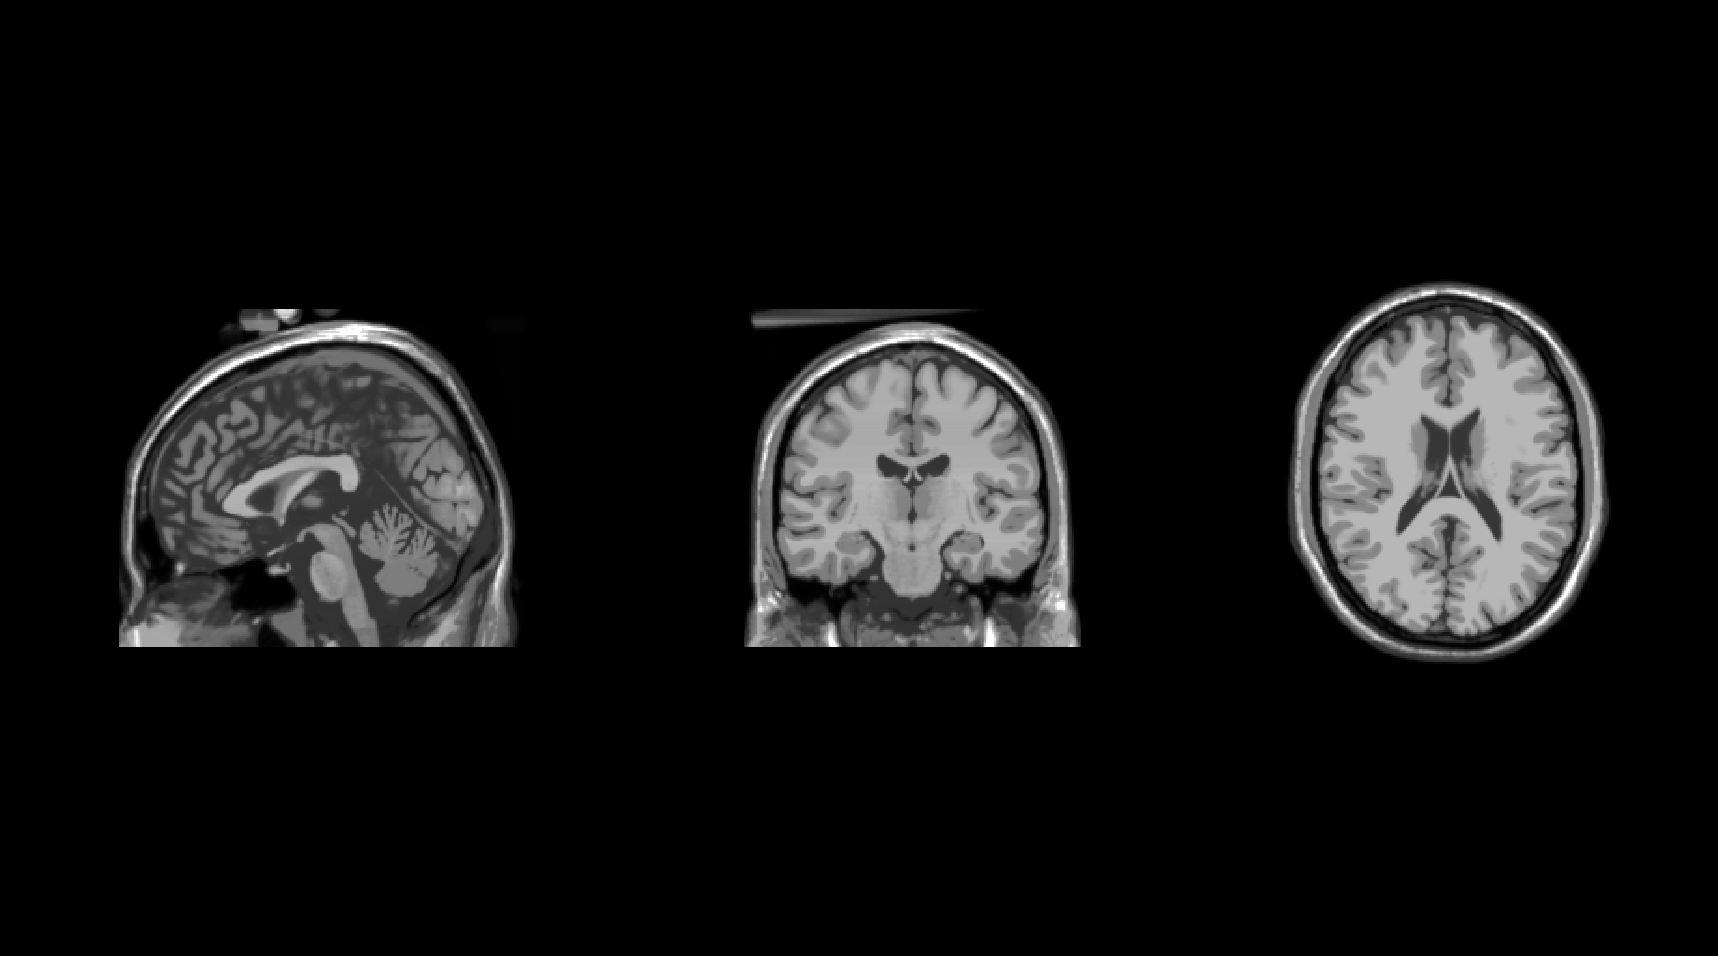
\includegraphics[width=\textwidth]{figuras/referenceImg.png}
      \subcaption*{(a)}
      \label{fig:refImg}
    \end{subfigure}
    \begin{subfigure}[t]{0.8\textwidth}
      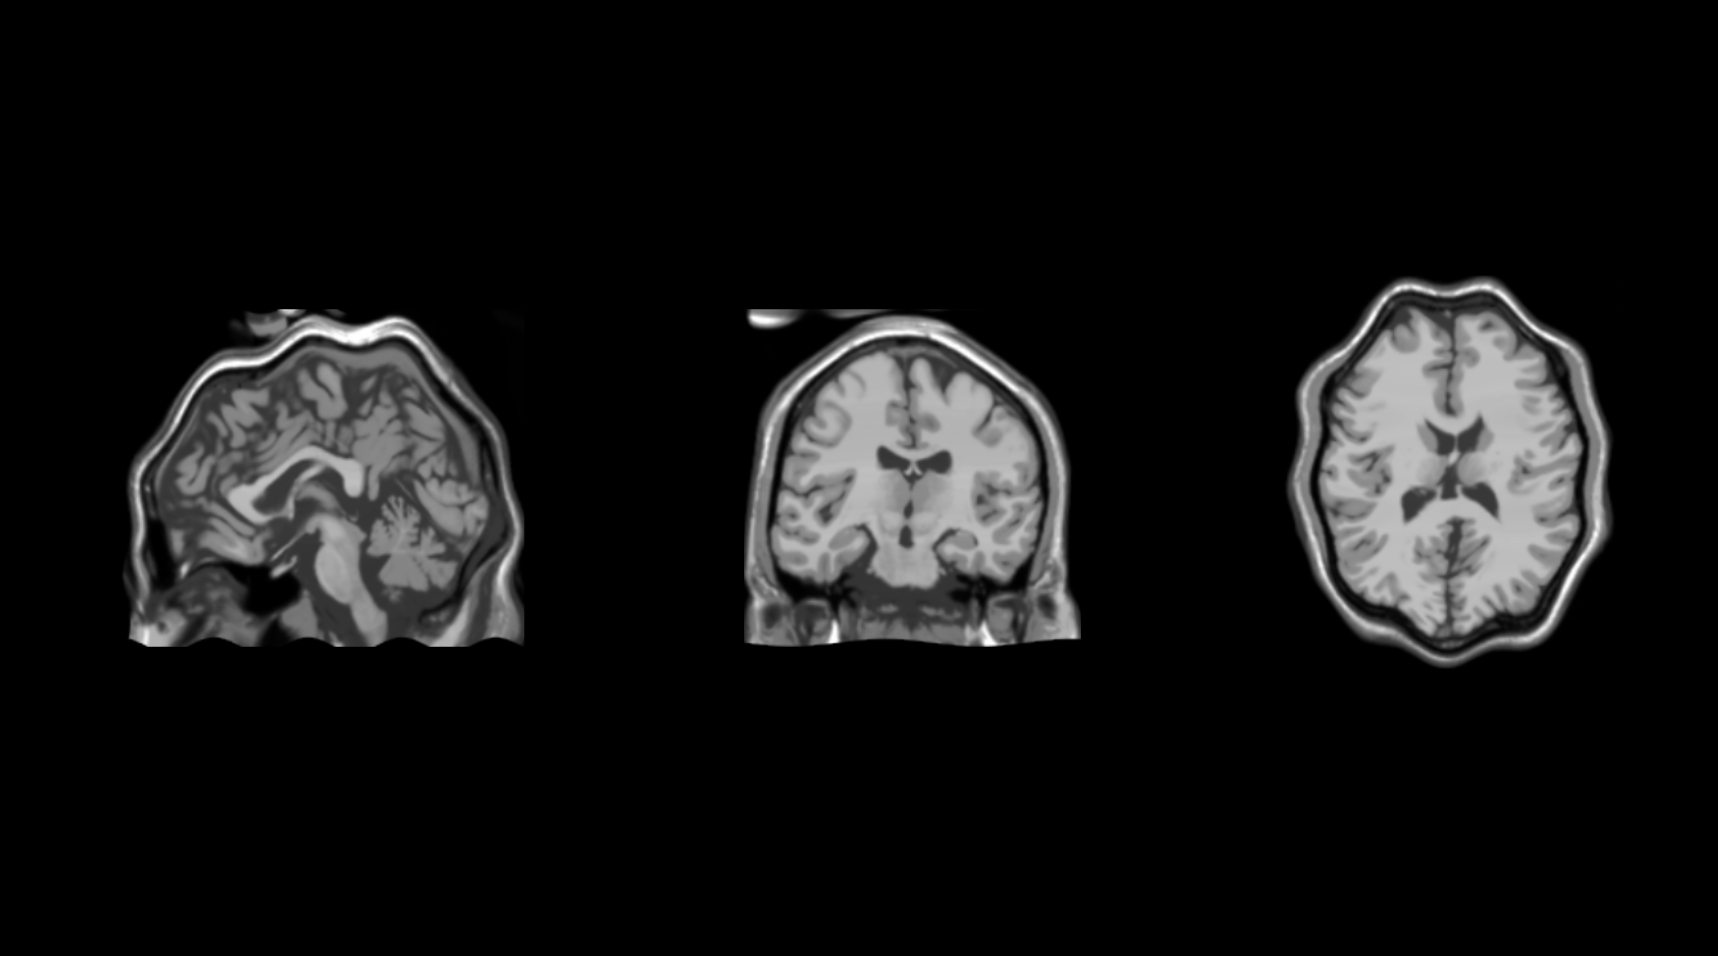
\includegraphics[width=\textwidth]{figuras/targetImg.png}
      \subcaption*{(b)}
      \label{fig:tarImg}
    \end{subfigure}
    \source{\cite{papademetris2005bioimage}}
    \caption{As imagens referência (a) e alvo (b) usadas nos experimentos.
             Na primeira coluna está o corte sagital, na segunda o corte
             coronal e por fim o corte axial.}
    \label{fig:testImg}
\end{figure}

\section{Resultados}

  Primeiramente, apresentamos os resultados de cada um dos quatro testes. As
imagem resultantes das quatro instâncias de registro não diferem quanto aos
experimentos, somente com o número de características. Elas são encontradas
na figura \ref{fig:resultsAll}.

\begin{figure}[H]
    \begin{minipage}[b]{0.45\linewidth}
      \centering
      \begin{subfigure}[t]{1\textwidth}
        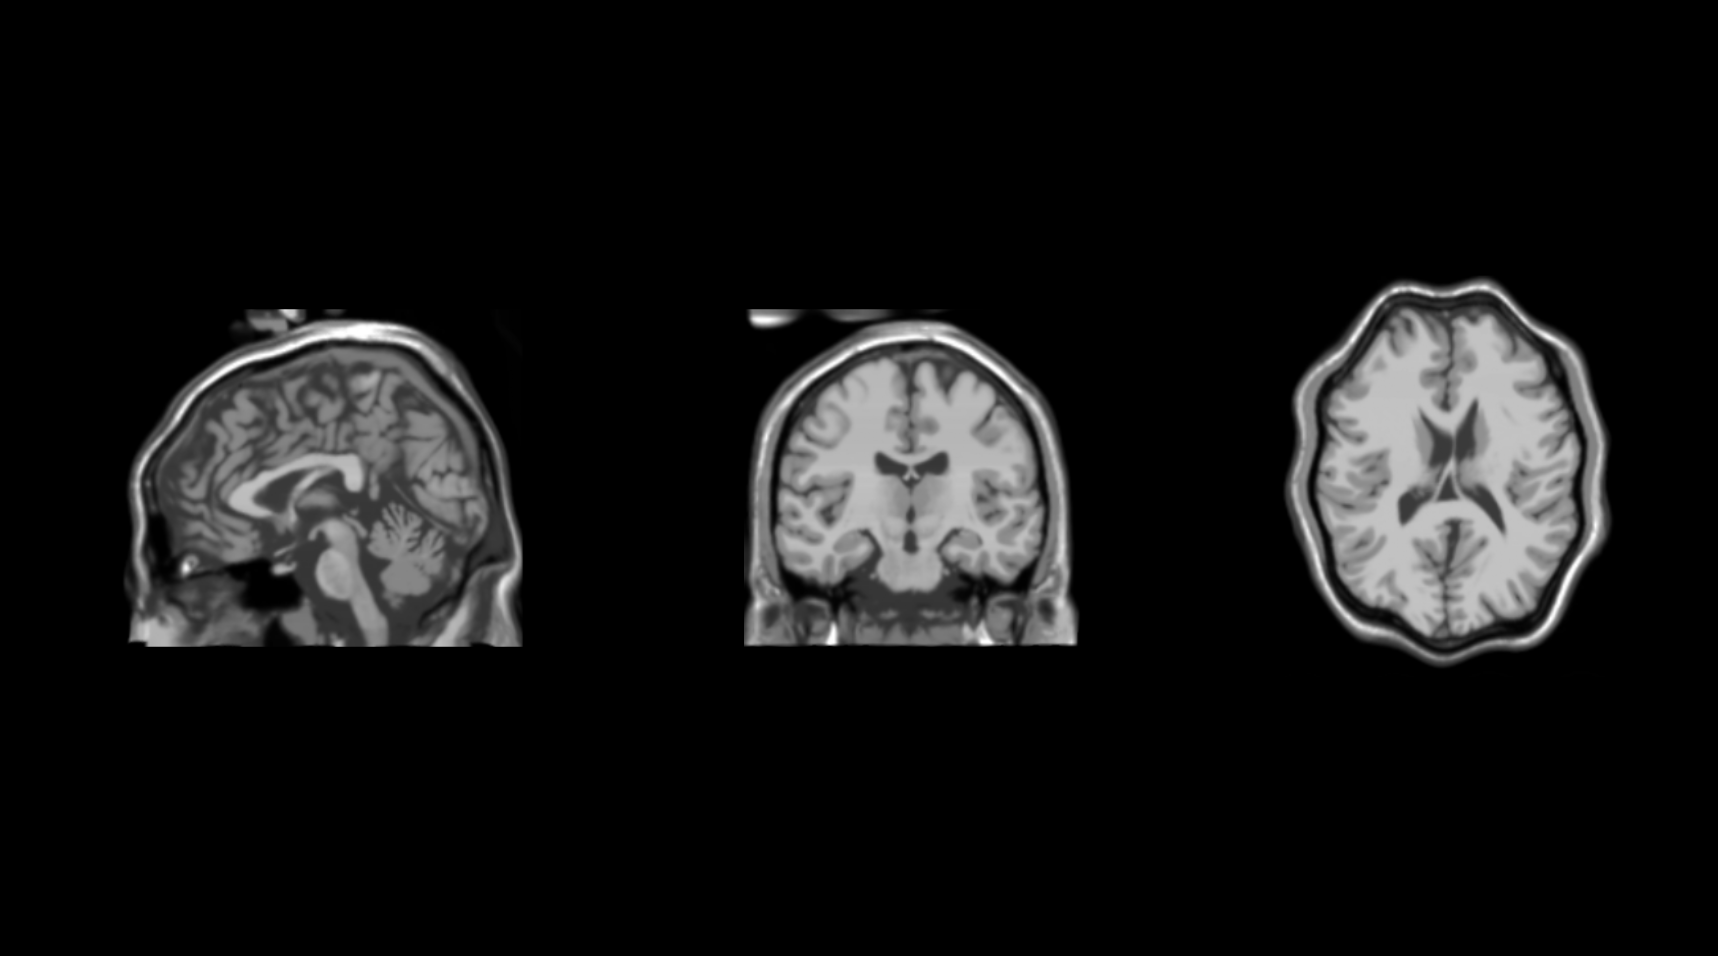
\includegraphics[width=\textwidth]{figuras/result001.png}
        \subcaption*{576 características.}
        \label{fig:576}
      \end{subfigure}
      \begin{subfigure}[t]{1\textwidth}
        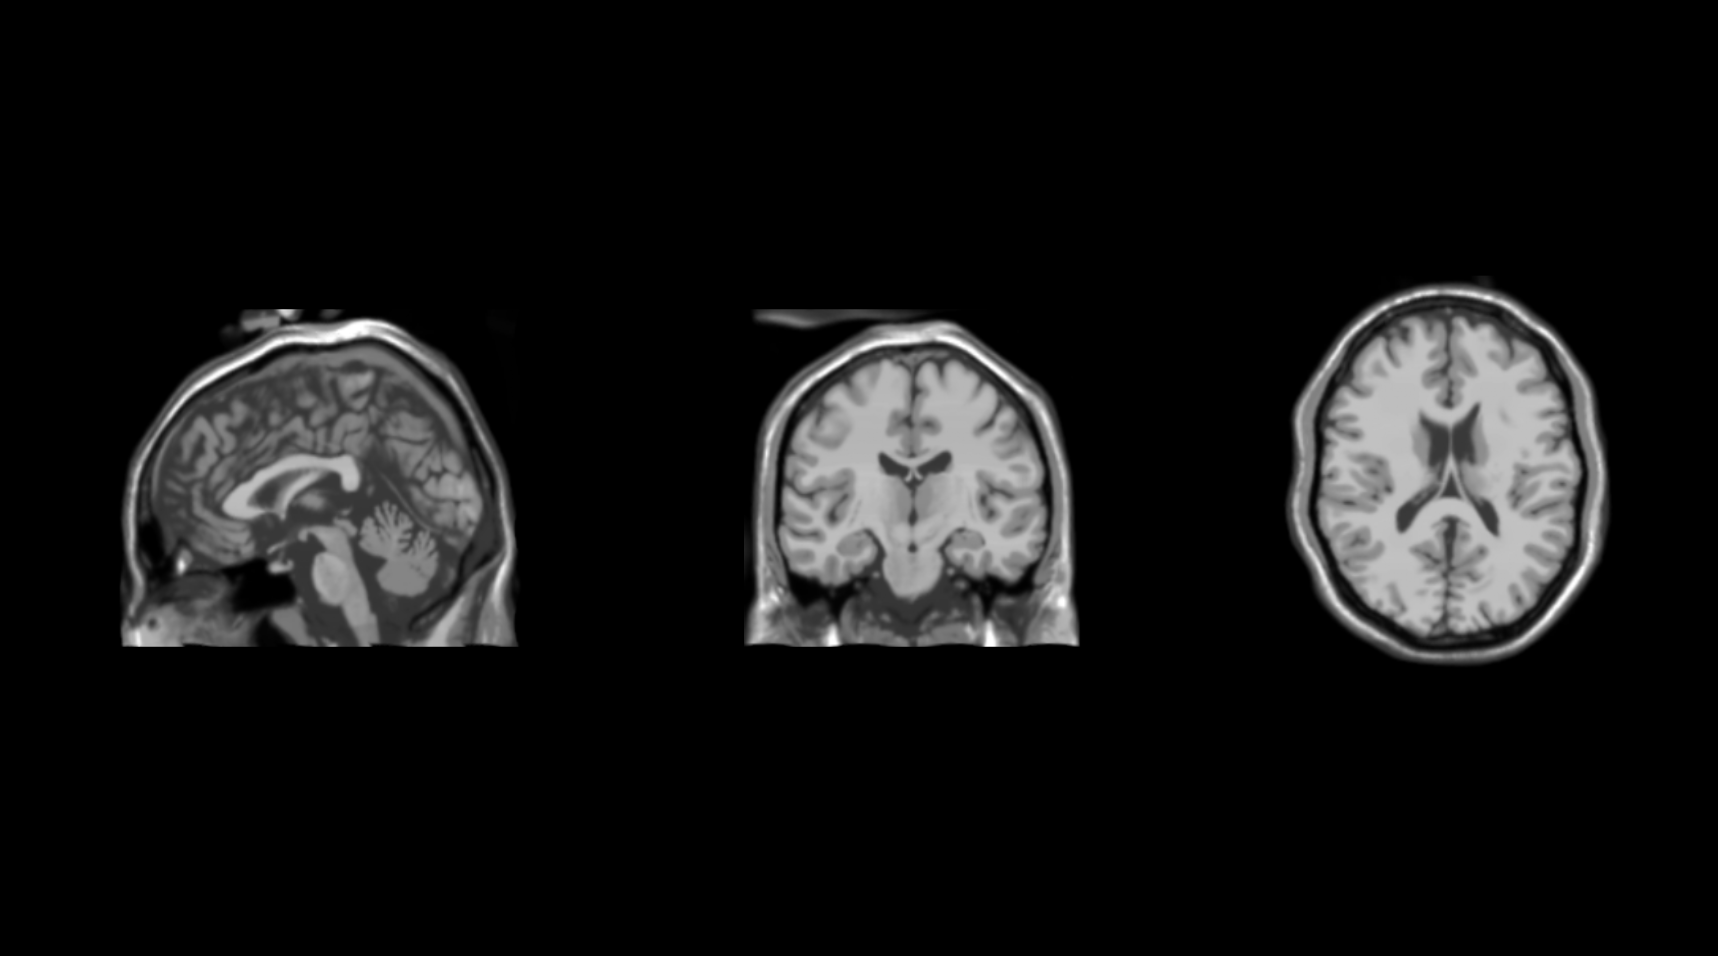
\includegraphics[width=\textwidth]{figuras/result002.png}
        \subcaption*{2016 características.}
        \label{fig:2016}
      \end{subfigure}
    \end{minipage}
    \hspace{0.5cm}
    \begin{minipage}[b]{0.45\linewidth}
      \centering
      \begin{subfigure}[t]{1\textwidth}
        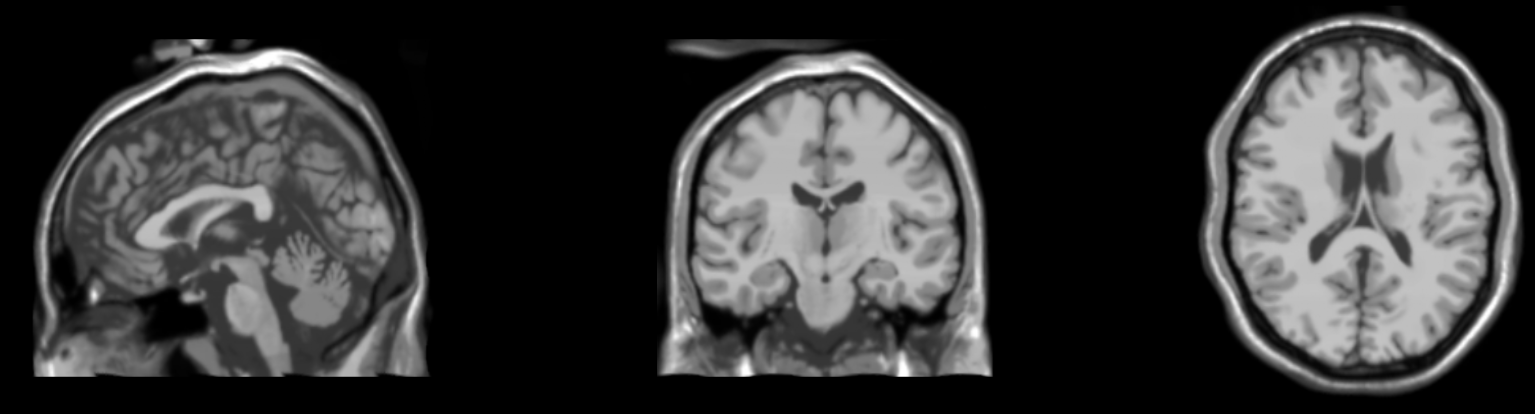
\includegraphics[width=\textwidth]{figuras/result003.png}
        \subcaption*{4864 características.}
        \label{fig:4864}
      \end{subfigure}
      \begin{subfigure}[t]{1\textwidth}
        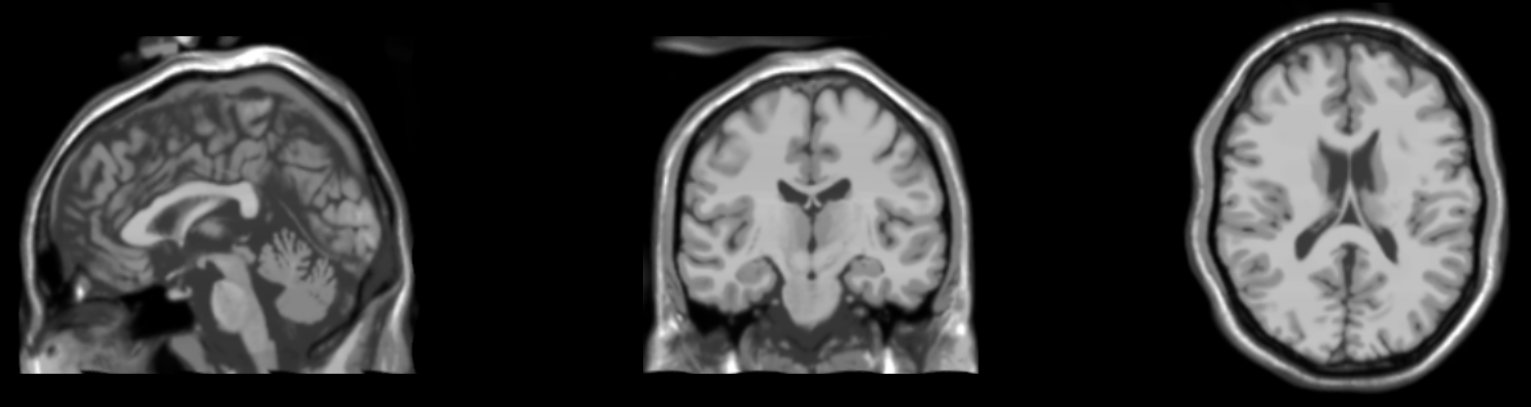
\includegraphics[width=\textwidth]{figuras/result004.png}
        \subcaption*{7942 características.}
        \label{fig:7942}
      \end{subfigure}
    \end{minipage}
    \caption{Resultado dos testes. A primeira coluna é um corte sagital,
             a segunda coluna um corte coronal e a última um corte axial.}
    \label{fig:resultsAll}
\end{figure}

  Para cada um dos oito experimentos, a média e desvio padrão do tempo de
execução dos trinta testes estão organizados na tabela \ref{table:resultsAll}.
A primeira parte da tabela mostra as métricas relacioandas ao método utilizado
para resolver o sistema linear enquanto a segunda parte apresenta as métricas
da execução do TPS juntamente com a interpolação trilinear. O TPS e a interpolação
estão juntos pois eles são executados dentro do mesmo kernel, o que melhora o
desempenho da implementação. Esses mesmos dados podem ser vistos nos gráficos
\ref{fig:chartTPS} e \ref{fig:chartSolver}.

% \begin{sidewaystable}
% \begin{tabular}{p{5em}|c|c|c|c|c|c|c|c|c|}
%     \cline{2-10}
%     & Pontos de controle
%     & \multicolumn{2}{|c|}{580}
%     & \multicolumn{2}{|c|}{2020}
%     & \multicolumn{2}{|c|}{4868}
%     & \multicolumn{2}{|c|}{7946}\\
%     \cline{2-10}
%     & Método
%     & Equação & TPS
%     & Equação & TPS
%     & Equação & TPS
%     & Equação & TPS\\
%     \hline
%     \multicolumn{1}{|c}{\multirow{2}{*}{CPU}}
%     & \multicolumn{1}{|c|}{Média (s)} & 0.193
%     & 276.071 & 7.346 & 960.756 & 96.722
%     & 2308.697 & 2582.082 & 3771.377 \\
%     \cline{2-10}
%     \multicolumn{1}{|c}{}
%     & \multicolumn{1}{|c|}{Desvio Padrão (s)}
%     & 0.0107 & 10.855 & 1.217 & 35.678
%     & 1.868 & 70.198 & 107.459 & 136.551 \\
%     \hline
%     \multicolumn{1}{|c}{\multirow{2}{*}{GPU sem melhorias}}
%     & \multicolumn{1}{|c|}{Média (s)} & 0.334
%     & 0.153 & 0.676 & 0.475 & 5.814 & 1.160
%     & 21.013 & 1.905 \\
%     \cline{2-10}
%     \multicolumn{1}{|c}{}
%     & \multicolumn{1}{|c|}{Desvio Padrão (s)}
%     & 0.009	& 0.003	& 0.013	& 0.002	& 0.077
%     & 0.003	& 0.184	& 0.005 \\
%     \hline
%     \multicolumn{1}{|c}{\multirow{2}{*}{GPU com calculadora de ocupação}}
%     & \multicolumn{1}{|c|}{Média (s)} & 0.343	& 0.162	& 0.679	& 0.503	& 5.826	& 1.227	& 20.975 & 2.012\\
%     \cline{2-10}
%     \multicolumn{1}{|c}{}
%     & \multicolumn{1}{|c|}{Desvio Padrão (s)}
%     & 0.024	& 0.003	& 0.014	& 0.001	& 0.066	& 0.001	& 0.241	& 0.002 \\
%     \hline
%     \multicolumn{1}{|c}{\multirow{2}{*}{GPU com textura}}
%     & \multicolumn{1}{|c|}{Média (s)} & 0.339	& 0.157	& 0.677	& 0.489	& 5.818	& 1.192	& 20.941 & 1.956\\
%     \cline{2-10}
%     \multicolumn{1}{|c}{}
%     & \multicolumn{1}{|c|}{Desvio Padrão (s)}
%     & 0.021	& 0.003	& 0.011	& 0.001	& 0.072	& 0.002	& 0.209	& 0.003\\
%     \hline
%     \multicolumn{1}{|c}{\multirow{2}{*}{GPU em paralelo}}
%     & \multicolumn{1}{|c|}{Média (s)} & 0.932	& 0.165	& 0.970	& 0.480	& 7.493	& 2.659	& 22.289	& 1.937\\
%     \cline{2-10}
%     \multicolumn{1}{|c}{}
%     & \multicolumn{1}{|c|}{Desvio Padrão (s)}
%     & 0.138	& 0.042	& 0.104	& 0.006	& 2.595	& 2.410	& 0.375	& 0.010\\
%     \hline
%     \multicolumn{1}{|c}{\multirow{2}{*}{GPU em paralelo e ocupação}}
%     & \multicolumn{1}{|c|}{Média (s)} & 0.998	& 0.159	& 0.962	& 0.509	& 7.480	& 1.866	& 22.317	& 2.047\\
%     \cline{2-10}
%     \multicolumn{1}{|c}{}
%     & \multicolumn{1}{|c|}{Desvio Padrão (s)}
%     & 0.144	& 0.010	& 0.103	& 0.006	& 2.437	& 1.622	& 0.473	& 0.012\\
%     \hline
%     \multicolumn{1}{|c}{\multirow{2}{*}{GPU com textura e ocupação}}
%     & \multicolumn{1}{|c|}{Média (s)} & 0.343	& 0.166	& 0.683	& 0.519	& 5.838	& 1.262	& 21.026	& 2.073\\
%     \cline{2-10}
%     \multicolumn{1}{|c}{}
%     & \multicolumn{1}{|c|}{Desvio Padrão (s)}
%     & 0.011	& 0.003	& 0.009	& 0.001	& 0.081	& 0.002	& 0.236	& 0.003\\
%     \hline
%     \multicolumn{1}{|c}{\multirow{2}{*}{GPU com textura em paralelo}}
%     & \multicolumn{1}{|c|}{Média (s)} & 0.971	& 0.160	& 0.967	& 0.492	& 8.803	& 2.154	& 22.310	& 1.992\\
%     \cline{2-10}
%     \multicolumn{1}{|c}{}
%     & \multicolumn{1}{|c|}{Desvio Padrão (s)}
%     & 0.101	& 0.028	& 0.090	& 0.004	& 2.978	& 1.974	& 0.301	& 0.010\\
%     \hline
%     \multicolumn{1}{|c}{\multirow{2}{*}{GPU com todas as melhorias}}
%     & \multicolumn{1}{|c|}{Média (s)} & 0.927	& 0.181	& 0.933	& 0.494	& 8.379	& 1.274	& 22.173	& 1.991\\
%     \cline{2-10}
%     \multicolumn{1}{|c}{}
%     & \multicolumn{1}{|c|}{Desvio Padrão (s)}
%     & 0.124	& 0.056	& 0.092	& 0.006	& 2.976	& 0.162	& 0.331	& 0.007\\
%     \hline
% \end{tabular}
% \end{sidewaystable}

\small
\begin{table}[H]
\begin{tabular}{l*{4}{c}}
    \toprule
    & \multicolumn{4}{c}{Características} \\
    \cmidrule(lr){2-5}
    Implementação & 576 & 2016 & 4864 & 7942\\
    \cmidrule(lr){1-1} \cmidrule(lr){2-5}
    \multicolumn{5}{c}{Solução do sistema linear} \\
    \midrule
    CPU & $0.193 \pm 0.011$ & $7.346 \pm 1.217$ & $96.722 \pm 1.868$ & $2582.082 \pm 107.460$\\
    GPU & $0.334	\pm 0.009$ & $0.676 \pm 0.013$ & $5.814 \pm 0.077$ & $21.012 \pm 0.183$ \\
    Calculadora de ocupação & $0.342 \pm 0.024$ & $0.678 \pm 0.014$ & $5.826 \pm 0.066$ & $20.975 \pm 0.241$\\
    Textura & $0.338 \pm 0.020$ & $0.676 \pm 0.011$ & $5.817 \pm 0.071$ & $20.940 \pm 0.209$ \\
    Paralelo & $0.932 \pm 0.138$	& $0.970 \pm 0.104$	& $7.492 \pm 2.594$	& $22.289 \pm 0.374$ \\
    Paralelo e ocupação & $0.997 \pm 0.144$ & $0.961 \pm 0.103$ & $7.480 \pm 2.436$ & $22.316 \pm 0.473$ \\
    Textura e ocupação & $0.342 \pm 0.011$ & $0.682 \pm 0.008$ & $5.837 \pm 0.080$ & $21.026 \pm 0.236$ \\
    Textura em paralelo & $0.971 \pm 0.101$ & $0.967 \pm 0.089$ & $8.803 \pm 2.978$ & $22.310 \pm 0.301$ \\
    Todas as melhorias & $0.926 \pm 0.124$ & $0.933 \pm 0.092$ & $8.379 \pm 2.975$ & $22.172 \pm 0.330$ \\
    \midrule
    \multicolumn{5}{c}{TPS/Interpolação} \\
    \midrule
    CPU & $276.071 \pm 10.855$ & $960.756 \pm 35.678$ & $2308.697 \pm 70.198$ & $3771.377 \pm 136.551$\\
    GPU & $0.152 \pm 0.002$ & $0.475 \pm 0.001$ & $1.159 \pm 0.003$ & $1.904 \pm 0.004$ \\
    Calculadora de ocupação & $0.161 \pm 0.003$ & $0.503 \pm 0.001$ & $1.226 \pm 0.001$ & $2.011 \pm 0.001$\\
    Textura & $0.156 \pm 0.002$ & $0.489 \pm 0.001$ & $1.192 \pm 0.002$ & $1.956 \pm 0.003$ \\
    Paralelo & $0.164 \pm 0.041$	& $0.480 \pm 0.005$	& $2.658 \pm 2.410$	& $1.936 \pm 0.009$ \\
    Paralelo e ocupação & $0.158 \pm 0.009$ & $0.508 \pm 0.006$ & $1.866 \pm 1.621$ & $2.047 \pm 0.011$ \\
    Textura e ocupação & $0.166 \pm 0.002$ & $0.519 \pm 0.001$ & $1.262 \pm 0.002$ & $2.072 \pm 0.002$ \\
    Textura em paralelo & $0.159 \pm 0.027$ & $0.492 \pm 0.003$ & $2.153 \pm 1.974$ & $1.992 \pm 0.010$ \\
    Todas as melhorias & $0.180 \pm 0.055$ & $0.494 \pm 0.006$ & $1.273 \pm 0.161$ & $1.991 \pm 0.006$ \\
    \bottomrule
\end{tabular}
  \caption{Tempo médio de execução das funções Solução do sistema linear e TPS/Interpolação.}
  \label{table:resultsAll}
\end{table}
\normalsize

\begin{figure}[H]
    \centering
      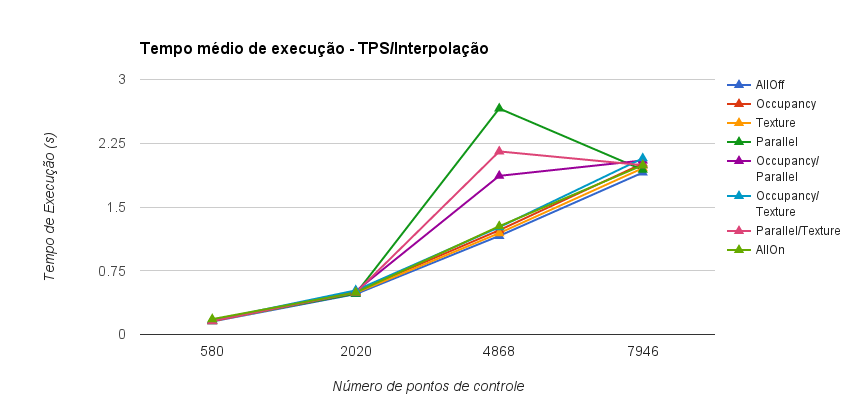
\includegraphics[width=1.1\textwidth]{figuras/chartTPS.png}
    \caption{Tempo médio de execução da funçãp TPS+Interpolação.}
    \label{fig:chartTPS}
\end{figure}

\begin{figure}[H]
    \centering
    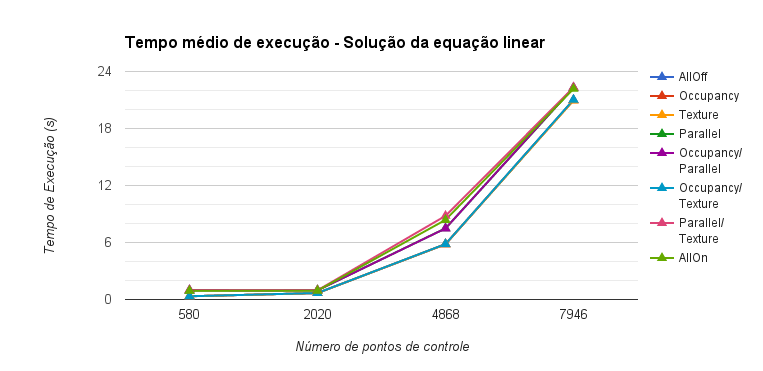
\includegraphics[width=1.1\textwidth]{figuras/chartSolver.png}
    \caption{Tempo médio de execução da função para resolver sistema linear.}
    \label{fig:chartSolver}
\end{figure}

  O ultimo conjunto de métricas geradas pelos experimentos é o tempo total de
execução das quatro instâncias de registro, levando em conta as três etapas do
registro. O gráfico \ref{fig:chartAverage} apresenta o tempo médio dos trinta
testes para cada um dos oito experimentos, com o desvio padrão representado
pelas colunas no fim de cada uma das barras.

\begin{figure}[H]
    \centering
    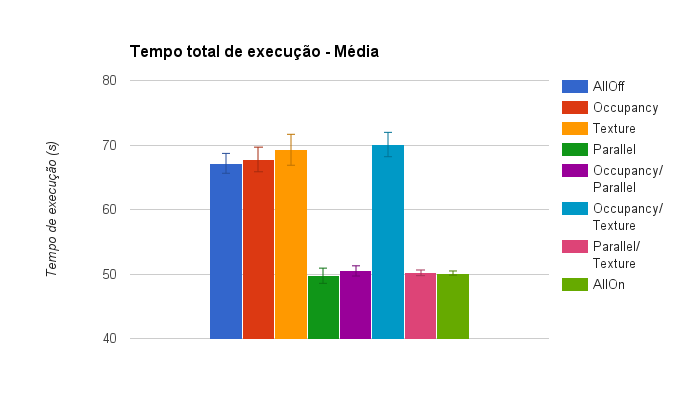
\includegraphics[width=1.1\textwidth]{figuras/chartAverage.png}
    \caption{Tempo médio de execução dos três passos do registro.}
    \label{fig:chartAverage}
\end{figure}

\begin{figure}[H]
    \centering
    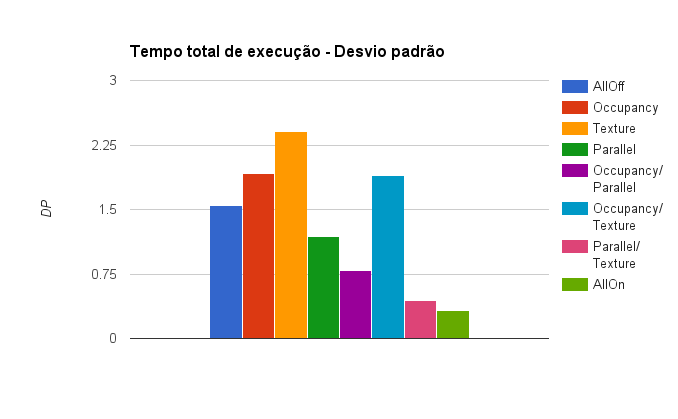
\includegraphics[width=1.1\textwidth]{figuras/chartDP.png}
    \caption{Desvio padrão do tempo de execução dos três passos do registro.}
    \label{fig:chartDP}
\end{figure}
